\documentclass[8pt,a4paper,landscape]{extarticle}

% -- Layout ----
\usepackage[top=0.5cm, bottom=0.5cm, left=0.5cm, right=0.5cm, landscape]{geometry}

% -- Titles ----
\usepackage[
  tiny,                     % text size title
  compact                   % reduce vertical space before/after title
]{titlesec}
% \titlespacing*
\titleformat{\section}{\normalfont\normalsize\bfseries}{\thesection}{0em}{} % Remove space before and after section titles
\titleformat{\subsection}{\normalfont\normalsize\bfseries}{\thesubsection}{0em}{} % Remove space before and after subsection titles
\titlespacing*{\section}{0pt}{0pt}{0pt} % Remove space before/after section titles
\titlespacing*{\subsection}{0pt}{0pt}{0pt} % Remove space before/after subsec titles

% -- Colors ----
\usepackage[dvipsnames,table]{xcolor}
% \definecolor{dim}{RGB}{192,192,192} % Define a custom dimmed text color
\definecolor{dim}{RGB}{240,240,245} % Define a custom dimmed text color
\definecolor{drow}{RGB}{248,249,250} % Define a custom dimmed text color
\definecolor{dmm}{RGB}{167,167,167} % Define a custom dimmed text color
\usepackage{soul}

% -- Math ------
\usepackage{mathtools}
\usepackage{amssymb}
\usepackage{pifont}

% -- Lists & tables -----
\usepackage[inline]{enumitem}
\setlist{noitemsep}% Remove vspace between items
% Set vspace before and after  list environments as well as the left margin
\setlist[itemize,1]{leftmargin=*,labelindent=1pt,topsep=1pt,partopsep=1pt}
\setlist[itemize,2]{leftmargin=2pt,labelindent=1pt,topsep=1pt,partopsep=1pt}
\setlist[enumerate,1]{leftmargin=*,labelindent=1pt,topsep=1pt,partopsep=1pt}
\setlist[enumerate,2]{leftmargin=1.2em,labelindent=1pt,topsep=1pt,partopsep=1pt}
\usepackage{multirow}

% Parse Trees
\usepackage{tikz}
\usetikzlibrary{ arrows, automata, bbox, calc, positioning }
\tikzset{
% ->, % makes the edges directed
>=stealth', % makes the arrow heads bold
node distance=1cm, % specifies minimum distance between two nodes
% small/.style={},
every state/.style={thick}, % sets the properties for each ’state’ node
every node/.style={inner sep=1pt},
initial text=start, % sets the text that appears on the start arrow
}

% Place a figure env right here via [H] option
\usepackage{float}

% Side by side figure
\usepackage{subcaption}

% -- Multi-Col layout --
\usepackage{multicol}


% No indentation
\setlength\parindent{0pt}

\newcommand{\mset}[1]{\(\{q_{#1}\}\)}
\renewcommand{\arraystretch}{1.2}
\newcommand{\xvdash}[1]{%
  \vdash^{\mkern-10mu\footnotesize\rule[-1.2ex]{0pt}{0pt}#1}%
}

\begin{document}
% Suppress page number for all pages
\pagestyle{empty}
% Math env spacing
\setlength{\abovedisplayskip}{1pt}
\setlength{\belowdisplayskip}{1pt}
\setlength{\abovedisplayshortskip}{0pt}
\setlength{\belowdisplayshortskip}{0pt}
% hl
\sethlcolor{dim}
% TODO:
% [] update anomalies
% [] ...
\begin{multicols*}{3}
\section*{Functional Dependencies (by E.F.Codd, 1971)}
\begin{minipage}{0.5\linewidth}
  \centering
  \begin{tabular}{c|ccccc}
    \hline
    \multicolumn{6}{c}{R($X_{i} \rightarrow Y_{i}$)}\\
    \hline
    & $X$ & $Y$ & $Z$ & $W$ & $U$ \\
    $t_{1}$ & $X_{1}$ & $Y_{1}$ & $Z_{1}$ & $W_{1}$ & $U_{1}$ \\
    & \multicolumn{5}{c}{\ldots}\\
    $t_{2}$ & $X_{2}$ & $Y_{2}$ & $Z_{2}$ & $W_{2}$ & $U_{2}$ \\
    \hline
    \multicolumn{6}{l}{$t_{1}[X_{i}] = t_{2}[X_{i}] \rightarrow t_{1}[Y_{i}] = t_{2}[Y_{i}]$}\\
    \hline
\end{tabular}
\end{minipage}
\begin{minipage}{0.5\linewidth}
  \centering
  \begin{tabular}{ccccc}
    \hline
    $A$ & $B$ & $C$ & $D$ & $E$ \\
    1 & 4 & 1 & 9 & 5 \\
    1 & 4 & 2 & 8 & 5 \\
    1 & 4 & 1 & 8 & 5 \\
    \hline
    \multicolumn{5}{l}{$AB \rightarrow E$}\\
    \multicolumn{5}{l}{$C \nrightarrow DE$}\\
    \hline
\end{tabular}
\end{minipage}

\begin{itemize}
% \item define \textbf{goodness} and \textbf{badness} of relational db design
% \item show \textbf{relationship} between and among attributes
\item top down: $R_{\text{schema}}$ + FDs \(\Rightarrow\) smaller schemas (normalization)
\item bottom up: $R_{\text{attrs}}$ + FDs $\Rightarrow$ $R_{\text{schema}}$ (not popular)
\item Attrs $A,B,C$ determine attrs $D,E$, written as:
  \begin{displaymath}
\{\underbracket[1pt]{A,B,C}_{\text{determinant}}\} \rightarrow \{\underbracket[1pt]{D,E}_{\text{dependent}}\}
\end{displaymath}
\item \textbf{trivial}: $\{A,B,C\} \rightarrow \{C\}$
\item \textbf{syntactical convention}: $ABC \rightarrow DE$
% \item  specify constraints that must hold at all times on a relation
\end{itemize}
\textbf{Theorem}\quad Given $\Sigma = \{FD_{1},\ldots,FD_{n}\}$, that $X \rightarrow Y$ is implied by $\Sigma$ is denoted as $\Sigma \models X \rightarrow Y$ and all possible FDs implied by $\Sigma$ is denoted as $\Sigma^{*}$.  If $\Sigma^{*}_{1} = \Sigma^{*}_{2}$, $\Sigma_{1}, \Sigma_{2}$ are equivalent

\begin{minipage}{\linewidth}
  \centering
  \begin{tabular}{l|c}
    \hline
    $\Sigma_{1} = \{ X \rightarrow Y, Y \rightarrow Z\}$ & $\{ X \rightarrow Y, Y \rightarrow Z, X \rightarrow Z\}$\\
    $\Sigma_{2} = \{ X \rightarrow Y, Y \rightarrow Z, X \rightarrow Z\}$ & $\{ X \rightarrow Y, Y \rightarrow Z, X \rightarrow Z\}$ \\
    \hline
    \multicolumn{2}{l}{$\because \Sigma^{*}_{1} = \Sigma^{*}_{2} \therefore \Sigma_{1}, \Sigma_{2}$ are equivalent but $\Sigma_{1} \neq \Sigma_{2}$ in this case}\\
    \multicolumn{2}{l}{if $\Sigma^{*}_{1} \neq \Sigma^{*}_{2}$, then $\Sigma_{1} \neq \Sigma_{2}$}\\
    \hline
\end{tabular}
\end{minipage}
\begin{minipage}{0.5\linewidth}
\begin{itemize}
\item \textbf{closure} of $X$ under $\Sigma$: $X^{+}$
\item $\Sigma \models X \rightarrow Y\; \mathsf{iff} \;Y \subseteq X^{+}$
\item \textbf{algorithm} of computing $X^{+}$
  \begin{enumerate}[leftmargin=0.5em]
  \item start with $X^{+} := X$
  \item\label{fd:clo1} if $X \rightarrow Y \in \Sigma$, add $Y$ to $X^{+}$
  \item\label{fd:clo2} for each $FD_{i}(\in \Sigma): A_{1} \rightarrow A_{2} $ if $A_{1} \subseteq X^{+}$, add $A_{2}$ to $X^{+}$
  \item[] $A_{1},A_{2}$ are both set of attrs
  \item repeat step \ref{fd:clo1} \& \ref{fd:clo2} until \textbf{no} changes on $X^{+}$
  \end{enumerate}
\end{itemize}
\end{minipage}
\begin{minipage}{0.5\linewidth}
$R = \{A,B,C,D,E,F\}$, $\Sigma_{R}=\{AC\rightarrow B,B\rightarrow CD, C \rightarrow E, AF \rightarrow B\}$, \hl{$\Sigma \models AC \rightarrow ED$?}
\begin{align*}
  (AC)^{+} & \subseteq AC && \text{initialisation}\\
           & \subseteq ACB && AC \rightarrow B\\
           & \subseteq ACBD && B \rightarrow CD\\
           & \subseteq ACBDE && C \rightarrow E\\
           & = ACBDE
\end{align*}
\[\because ED \subseteq (AC)^{+},\;\therefore \Sigma \models AC \rightarrow ED\]
\end{minipage}

\section*{Finding [Candidate] Keys (FD closure)}
\begin{minipage}{\linewidth}
  \begin{tabular}{r|l|l}
    \hline
    Key & Def & Range\\
    \hline
    Super & uniquely determin all attrs of $R$ & $SK \subseteq R_{\text{attrs}}$ \\
    Candidate & $\nexists CK_{i} \subset CK \equiv SK $ & $CK_{i} \subset CK \subset SK$\\
    Primary & chosen from candidate keys & $PK \subset CK$\\
    \hline
    \multicolumn{3}{l}{to find a key is to find a candidate key (aka. \textbf{keys})}\\
    \hline
\end{tabular}
\end{minipage}
\begin{minipage}{0.5\linewidth}
\vspace{0.2em}
\begin{enumerate}
\item for each $X \subseteq R$, compute: $(A)^{+},\ldots,(Z)^{+},(AB)^{+},\ldots$
\item if $(X)^{+} = R$, $X$ is a superkey,
\item if $\nexists (Y\subset X)^{+} = R$, x is a key
\item Attrs in key: \textbf{prime}
\item Attrs \emph{not} in key \textbf{non-prime}
\end{enumerate}
\end{minipage}
\begin{minipage}{0.5\linewidth}
$R=\{ABCD\}$, $\Sigma=\{AB\rightarrow C, AC\rightarrow D\}$, \hl{find superkey?}
\[
(A)^{+}=A,(B)^{+}=B,(C)^{+}=C,\ldots
\]
\[
(AB)^{+}=ABCD,(AC)^{+}=ACD,\ldots
\]
\[
(ABC)^{+}=ABCD,(ABD)^{+}=ABCD\ldots
\]
key: $AB$, superk: $AB[CD]\{2\}$
\end{minipage}
\begin{minipage}{0.5\linewidth}
\begin{enumerate}
\item\label{fd:key1} if $A$ never shows in RHS of any FD, $A$ must be part of each key
\item[]$R=\{ABCD\}$, $\Sigma=\{C\rightarrow D, AB\rightarrow C, D\rightarrow A\}$, $B$ must be part of each key (\ref{fd:key1})
\item\label{fd:key2} if $A$ never shows in LHR det. of any FD but in RHS of any FD, $A$ must \emph{not} be part of each key
\item if $\exists X_{A} \subset A$ is a key, $A$ must \emph{not} be a key
\end{enumerate}
\end{minipage}
\begin{minipage}{0.47\linewidth}
$R=\{ABCDE\}$, $\Sigma=\{AE\rightarrow BC, B\rightarrow A, AB\rightarrow DE, C\rightarrow A\}$
\begin{itemize}
\item $D$ must \emph{not} be in each k (\ref{fd:key2})
\item  $(B)^{+} = ABCDE$, $B$ is a key
\item  $(A_{1}A_{2})^{+}$ \emph{without} $B$ e.g. $(AE)^{+}$
\item  $(A_{1}A_{2}A_{3})^{+}$ \emph{without} $B$ e.g. $(ACD)^{+}$
\item do \emph{not} comp. each $(FD_{\text{LHS}})^{+}$
\end{itemize}
\end{minipage}

\section*{Normal Forms (from weak to strong/more restrictive)}
\begin{minipage}{\linewidth}
\begin{tabular}{l|l|l|l}
  \hline
  NF & \multicolumn{3}{l}{Trait}\\
  \hline
  \textcolor{dmm}{1NF} & \multicolumn{3}{l}{\textcolor{dmm}{$R_{\text{attrs}}$ are all single type values (int,str,etc.); not relations}}\\
  \textcolor{dmm}{2NF} & \multicolumn{3}{l}{\textcolor{dmm}{FD $\geq 1$ where $CK \rightarrow A_{\text{non-prime}}$}}\\
  3NF & \multicolumn{3}{l}{All non-trivial FDs: $CK \rightarrow A_{\text{ttrs}}\;|\; X_{\text{attr(s)}} \rightarrow A_{\text{prime}}$}\\
  BCNF &  \multicolumn{3}{l}{All non-trivial FDs: $CK \rightarrow A$}\\
  \hline
  \multicolumn{4}{l}{It's important to find (candidate) keys ($SK$/$CK$ , aka. keys) first}\\
  \multicolumn{4}{l}{Prime attributes $\subseteq CK$}\\
  \hline
  \multicolumn{4}{l}{Normalization of $R$ is to decompose $R$ into $R_{\text{smaller}}$ in 3NF/BCNF}\\
  \hline
     & loss-less join & dependency preserving & no anomalies\\
  3NF & \ding{51}  & \ding{51} & \ding{55} (data redundy.)\\
  BCNF &\ding{51} & \ding{55} & \ding{51}\\
  \hline
\end{tabular}
\end{minipage}

\section*{Minimal Cover/Basis (Normalization to 3NF)}
\begin{minipage}{0.5\linewidth}
\begin{enumerate}
\item\label{item:5} find all candidate keys
\item find minimum cover
\begin{enumerate}[leftmargin=0pt]
\item[a.] make each $X\rightarrow \{A_{1},\ldots A_{k}\}$ to
\item[] $X\rightarrow A_{1}\ldots X\rightarrow A_{k}$
\item[b.] each FD has as few LHS $A$s as possible
\item[]check each $B \in X$, if $(X-B) \rightarrow A$?
\end{enumerate}
\item create a $R$ for each FD in min cover
\item create a $R$ for each $CK$ not yet in $Rs$ of step 3
\end{enumerate}
\end{minipage}
\begin{minipage}{0.5\linewidth}
$\Sigma=\{A\rightarrow B,ABCD\rightarrow E,EF\rightarrow GH,ACDF\rightarrow EG\}$
\begin{enumerate}
\item each FD has ONLY 1 RHS $A$ and get a new FDs set $\Sigma'$
  \begin{enumerate}[leftmargin=2pt]
  \item[a.] $EF\rightarrow G,EF\rightarrow H$\ldots
  \end{enumerate}
\item remove redundant FDs in $\Sigma'$
  \begin{enumerate}[leftmargin=2pt]
  \setcounter{enumi}{2}
  \item[b.] A\st{B}CD due to $A^{+} = AB$ and $ABCD^{+}=ABCDE$
  \item[a.] $ACD\rightarrow E$ cancels $ACDF\rightarrow E$
  \end{enumerate}
\item minimal cover always exists but not necessarily unique
\end{enumerate}
\end{minipage}

\section*{Normalization to BCNF}
\[
R=\{ABCD\}, CK = ABC, \Sigma=\{ABC\rightarrow D,D\rightarrow A\}
\]

\begin{minipage}{0.5\linewidth}
\begin{enumerate}
\item find FDs violating BCNF
\item decompose each such FD
\item[] $X\rightarrow A$ to $R-X$ and $XA$
\item repeat until all $R$s meet BCNF
\end{enumerate}
\end{minipage}
\begin{minipage}{0.5\linewidth}
\begin{enumerate}
\item $D\rightarrow A$ violates, decompose
\item to $R_{1}(AD)$, $R_{2}(BCD)$
\item[] $X\rightarrow A$ to $R-A$ and $XA$
\item repeat until all $R$s meet BCNF
\end{enumerate}
\end{minipage}

\section*{Query Optimization}
\begin{minipage}{0.5\linewidth}
\begin{enumerate}
\item Semantic query optimization
\item Rule-based query optimization
\item Cost-base query optimization
\end{enumerate}
\end{minipage}
\begin{minipage}{0.5\linewidth}
\begin{enumerate}
\item Push down selection
\item Push down projection
\item Re-order joins
\end{enumerate}
\end{minipage}

\section*{Heuristic Rules}
\begin{minipage}{\linewidth}
\begin{enumerate}[leftmargin=4em]
\item $\sigma_{\varphi}(\sigma_{\psi}(R))\equiv\sigma_{\varphi\wedge\psi}(R)$
\item $\pi_{X}(\pi_{Y}(R))\equiv\pi_{X}(R)$ if $X \subseteq Y$
\item $\sigma_{\varphi}(R_{1}\times R_{2})\equiv R_{1}\bowtie_{\varphi} R_{2}$
\item $\sigma_{\varphi1}(R_{1}\bowtie_{\varphi2} R_{2})\equiv R_{2}\bowtie_{\varphi1\wedge\varphi2} R_{1}$

\item $\sigma_{\varphi}(R_{1}\bowtie R_{2})\equiv\sigma_{\varphi}(R_{1})\bowtie R_{2}$
\item[] if $\varphi$ contains only attrs in $R_{1}$
\item $\sigma_{\varphi1\wedge\varphi2}(R_{1}\bowtie R_{2})\equiv\sigma_{\varphi1}(R_{1})\bowtie\sigma_{\varphi2}(R_{2})$
\item[] if $\varphi1$ contains only attrs in $R_{1}$; $\varphi2$ contains attrs only in  $R_{2}$
\item $\pi_{X}(R_{1}\bowtie R_{2})\equiv \pi_{X_{1}}(R_{1})\bowtie \pi_{X_{2}}(R_{2})$
\item[] join condition contains only attrs in $X$
\item $\pi_{X}(R_{1}\bowtie R_{2})\equiv \pi_{X}(\pi_{X_{1}}(R_{1})\bowtie \pi_{X_{2}}(R_{2}))$
\item[] join condition contains attrs not in $X$
\end{enumerate}
\end{minipage}

\section*{SQL Security (objects, threats \& ctrl measures)}
\begin{minipage}{\linewidth}
  \centering
  \begin{tabular}{r|l}
    \hline
    Objects & Threats \\
    \hline
    Confidentiality & illegitimate access (std can view others' grades)\\
    Integrity & data corruption (std can modify their grades)\\
    Availability & inaccessible (lecturer can't modify std' grades)\\
    \hline
\end{tabular}
\end{minipage}
\begin{minipage}{0.5\linewidth}
\begin{itemize}
\item Access, restrict access privileges
  \begin{itemize}
  \item authentication (passwd,PIN...)
  \item authorization (privilege level)
  \item other measures (IP restrct.)
  \end{itemize}
\item Inference, can't infer data statistically (avg $\nrightarrow$ particular)
\item Flow, data $\overset{flow}{\nrightarrow}$ unauthorized
\item Encryption, protect sensitive data
\end{itemize}
\end{minipage}
\begin{minipage}{0.5\linewidth}
\begin{enumerate}
\item Discretionary access ctrl (DAC)
  \begin{itemize}
  \item based on access privileges
  \item support: SQL + DBMS$_{\text{most}}$
  \end{itemize}
\item Mandatory access ctrl (MAC)
  \begin{itemize}
  \item various data sensitivity level
  \item support:  DBMS$_{\text{some}}$
  \end{itemize}
\item Row-based access ctrl (RBAC)
  \begin{itemize}
  \item users grouped by roles
  \item support: SQL + DBMS$_{\text{many}}$
  \end{itemize}
\end{enumerate}
\end{minipage}

\section*{Transactions (seq of db grouped operations)}
\begin{minipage}{0.5\linewidth}
ACID properties of db transactions
\begin{enumerate}
\item \textbf{A}tomicity each tx is atomic
\item[]ALL/NONE completed (central)
\item \textbf{C}onsistency
\item[]db st. consistent before/after tx
\item \textbf{I}solation
\item[] tx not affected by concurrency
\item \textbf{D}urability
\item[] tx done has persist effects in db
\end{enumerate}
\end{minipage}
\begin{minipage}{0.5\linewidth}
Concurrency ctrl to avod 4 problems
\begin{enumerate}
\item lost update (write-write conflt.)
\item[] 2 txs update same object
\item dirty read (write-read conflt.)
\item[] tx$_{1}$ reads obj uncommited by tx$_{2}$
\item un-repeated read (read-write)
\item[] tx$_{1}$ reads in-progress objs (tx$_{2}$)
\item phantom read
\item[] txs get diff rets at diff times
\end{enumerate}
\end{minipage}

\section*{Relational Algebra (6 operators makes a complete set)}
\begin{minipage}{0.5\linewidth}
\begin{enumerate}
\item selection $\sigma$
\item projection $\pi$
\item renaming $\rho$
\end{enumerate}
\end{minipage}
\begin{minipage}{0.5\linewidth}
\begin{enumerate}[resume,start=3]
\item union $\cup$
\item difference –
\item Cartesian product $\times$
\end{enumerate}
\end{minipage}
\begin{minipage}{\linewidth}
\begin{enumerate}
\item \textbf{not}, \textbf{never}, \textbf{only}, \textbf{always}, \textbf{exactly} indicates use of difference -
\item ``never''
  \begin{enumerate}[leftmargin=2pt]
  \item[a] Find all the (combinations of) tuples that are involved.
  \item[b] Use difference to subtract those that have occurred.
  \end{enumerate}
\item ``only'' and ``always''
  \begin{enumerate}[leftmargin=2pt]
  \item[a] Find all the (combinations of) tuples that are involved.
  \item[b] Use difference to subtract those that didn’t always occur.
  \end{enumerate}
\end{enumerate}
\end{minipage}

\section*{Query Tree}
\begin{minipage}{0.55\linewidth}
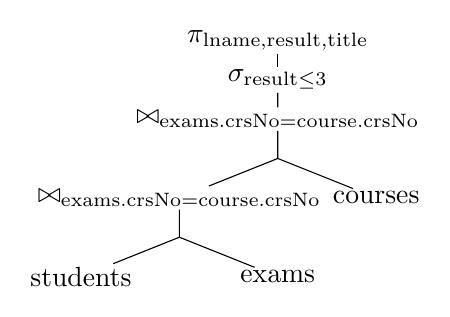
\begin{tikzpicture}[level distance=5mm,level/.style={sibling distance=2.5cm}]
  \node {$\pi_{\text{lname,result,title}}$}
  child {
      node {$\sigma_{\text{result}\leq 3}$}
      child {
        node {$\bowtie_{\text{exams.crsNo}=\text{course.crsNo}}$}
        child {
          child {node {$\bowtie_{\text{exams.crsNo}=\text{course.crsNo}}$}
            child {
              child {node {students}}
              child {node {exams}}
            }
          }
          child {node {courses}}
        }
      }
    };
\end{tikzpicture}
\end{minipage}
\begin{minipage}{0.45\linewidth}
\begin{itemize}
\item leaf nodes: input relations
\item internal nodes: intermediate result
\item root nodes: resulting relations
\end{itemize}
\end{minipage}

\section*{Enhanced Entity Relational Diagram}
\begin{figure}[H]
  \centering
  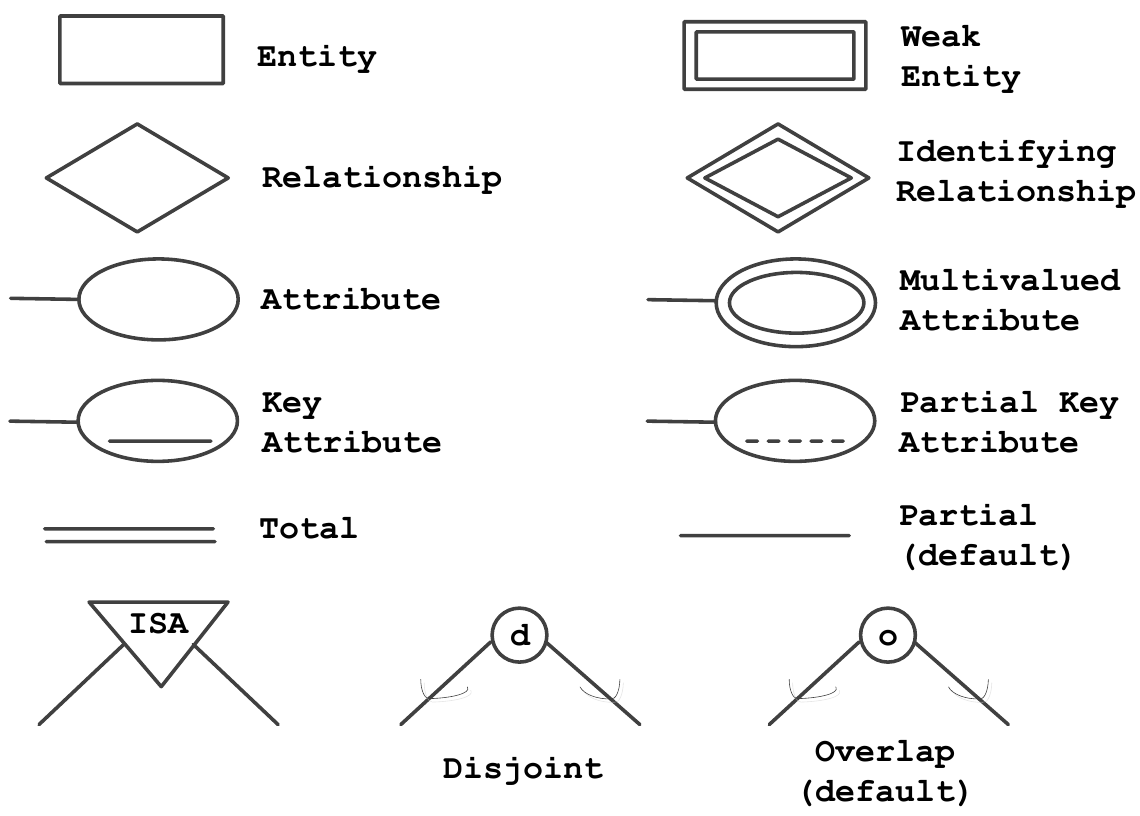
\includegraphics[width=0.75\linewidth]{eer.png}
  % \caption{Notations for EER diagrams}
  \label{fig:example}
\end{figure}
\end{multicols*}
\end{document}
